\cleardoublepage
\chapter{Implementation}
\label{ch:implementation}
Chapter 4 describes the implementation of the thesis.
This includes how the thesis group chose to implement the design discussed in previous chapters, and the research methods used to arrive at design decisions.

\section{REST API}\label{sec:REST API}

The API is a REST API coded in C\# with .NET.
REST stands for REpresentational State Transfer and is a software architecture style.
For the API to be considered a REST API it has to follow some set guidelines and principles.

The API consists of 4 different modules: The API endpoints, DataAccess,\\
DataAccess.Maintenance and Model.

\textbf{API endpoints} contains the controllers which handles the routing and requests.
There are three controllers, one for receipt, one for image and one for connecting to the machine learning API\@.
They receipt and image contain the methods GET, POST, PUT, and DELETE\@.
While the machine learning only contains on  for posting a picture.

In ImagesController the POST method uses the ImageDTO object.
It initializes a new Image object, and populates the corresponding data.
To set the image data, it serializes the image data from the DTO, and uses this data to for the image data.

\textbf{DataAccess} contains the DataContext for the database.
For the sake of simplicity, we have decided to utilize a local database.

\textbf{DataAccess.Maintenance} contains the migrations for the project.
This is to make it cleaner and to have a console app where it is possible to update the database without having to run the API\@.

The \textbf{Model} module contains the different models we use.
There is one for receipts and one for image, there is also a data transfer object for image.
The DTO is an object that carries data between processes and makes it more efficient by doing it in only one call.
This is done by aggregating the data instead of sending it one by one.


\section{ML API}\label{sec:ML API ch4}
The ML API is created using Flask.
This has one POST route that takes in an base64 string and converts it to an image and sends it to CNN and OCR for
processing.
The data is then returned to the .NET API

\section{Web solution}\label{sec:Web solution}

The web solution is made with React in JavaScript.
The purpose of the web solution is to give the user an interface where they can upload an image of a receipt.
And get the corresponding data from the image, and then send in the receipt with the data from the image.
This is to make the process of entering the data less time consuming.

When the user uploads an image, the web solution sends a POST request to the API, then the API saves the image to
the database.
When the image is saved, the image is sent to the OCR for text recognition.
If the output makes sense the data is returned and displayed to the user.
Then if the returned data is correct the user can then upload the receipt to the database.

\section{Dataset}\label{sec:dataset2}

As mentioned previously, dataset provided by Simployer consists of 1194 unlabeled images and PDF's.
However, the variance of the types of receipts in the dataset is very large.
When attempting to label the data with the corresponding company name, the amount of different companies were very large.
Because of this, we end up with a very small amount of images of each type after labeling them.
We decided to use the 3 most frequent companies, with the third most frequent company occurring only 19 times.
At the end of this process, the amount of usable data was very small.
The original dataset of 1194 images has been filtered down to 91 images, split into three different types of receipts.

\begin{figure}[h]
    \center{\includegraphics[width=1\textwidth]{Images/exampleimages}}
    \caption{Examples of labeled images}
    \label{fig:figure4.1}
\end{figure}

\section{Pre-processing}\label{pre-processing}

\subsection{Aligning}\label{aligning}

The first thing we make sure to do in our OCR is aligning the images.
This is needed because an OCR can't reed skewed images.
This means that we need to horizontal align the text as well as possible.

\subsubsection[aligning]{Matching}

Matching is a good way of having a dynamic aligning algorithm.
We have template images for all the different receipts types (in this case 3 images).
What the matching algorithm does is to look through the receipt you feed it and see if it has any "mathces" with the template one.
It then calculates how much it needs to skew the image in a given direction, to make it aligned with the template version.

\begin{figure}[h]
    \center{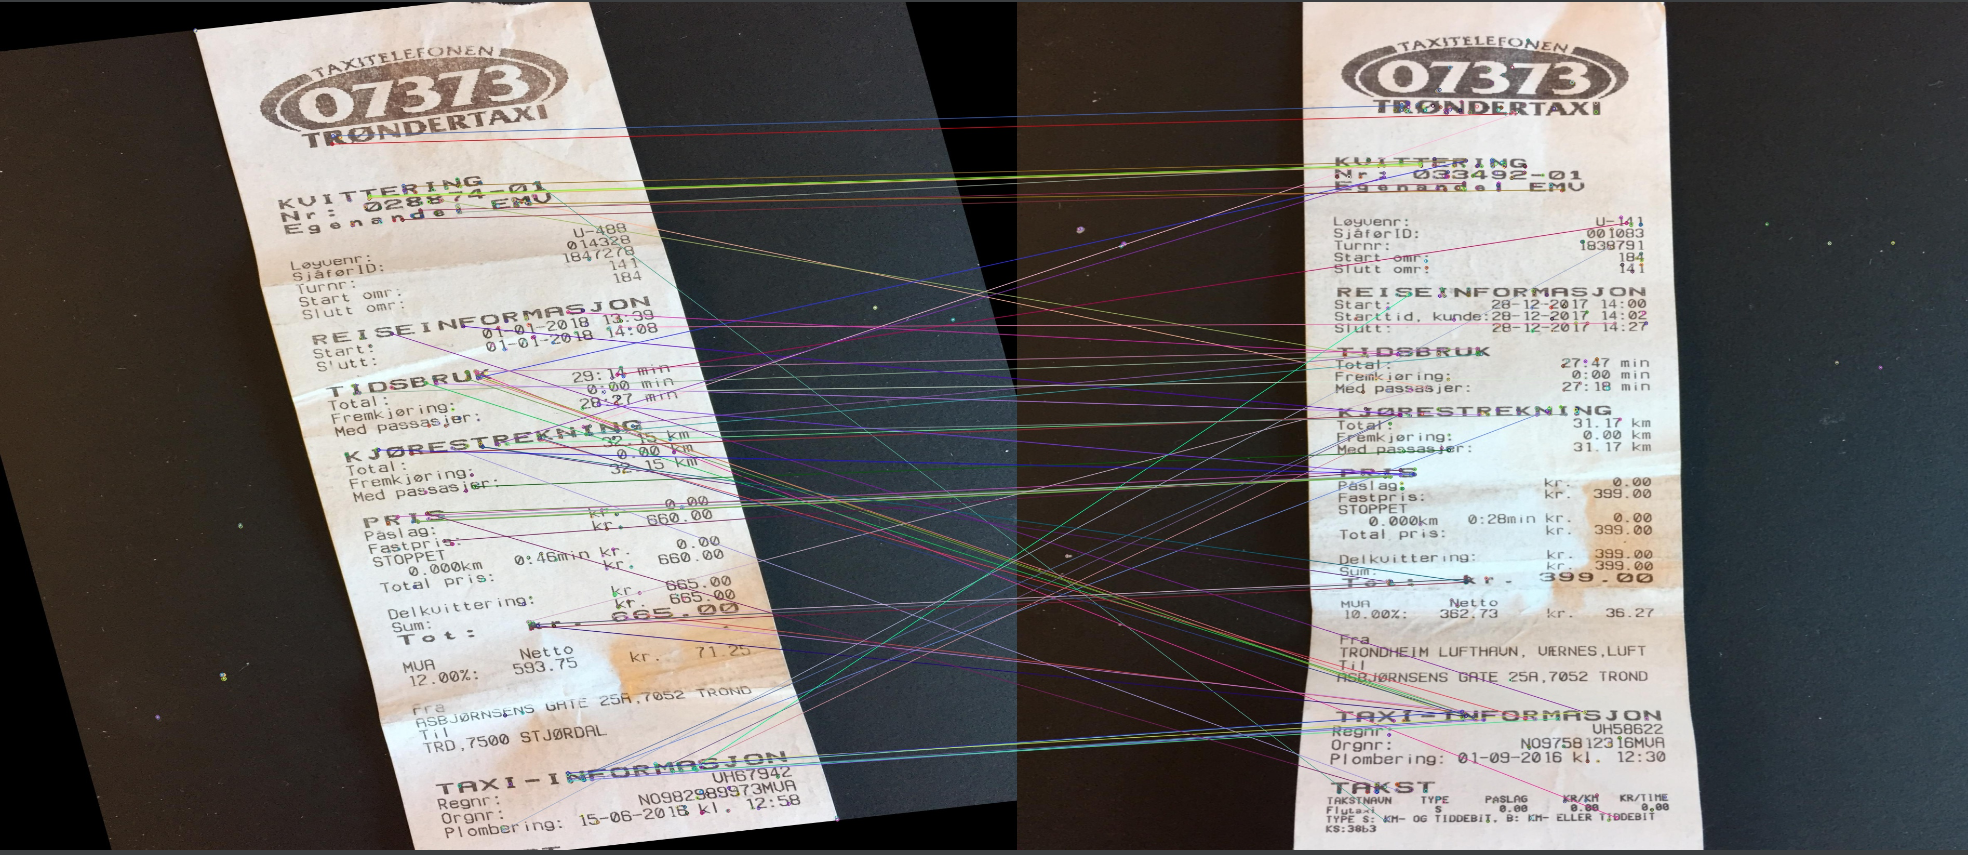
\includegraphics[width=1\textwidth]{Images/match_image.png}}
    \caption{Finding matches between a given image to a template}
    \label{fig:OCR matching}
\end{figure}

In image \ref{OCR matching} you can see the algorithm finding matches between a Trøndertaxi receipt from two different years.
Yes, these recipes is almost identical.
Making this functionality dynamic for almost all receipts should be possible, (no evidence for this) by having a pool of template receipts.
Then you can have a CNN check which receipts are the most similar and use the highest scoring receipt as the template image for any given receipt.

\subsection{Data augmentation}\label{data augmentation}
Because of the low amount of images in the filtered dataset, data augmentation has to be done in order to give us enough images to be able to effectively train the CNN.
We used an open source data augmentation tool for images for this task LINK.
The augmentor takes a directory of images and applies a series of transformations on the images like scaling, skewing and rotating.
This creates copies of the images with slight differences, increasing the size of our dataset.
After applying enough transformations, the size of the dataset grew from 91 images to 1500.

\begin{figure}[h]
    \center{\includegraphics[width=1\textwidth]{Images/example_augmented}}
    \caption{Original image on the left, along with generated images from blur and rotation transformations}
    \label{fig:figure4.3}
\end{figure}

\subsection{Image preparation}\label{imgprep}
Many of the images in the dataset are taken in different resolutions.
In order to prepare the images to be passed forward to the CNN model, the images resolution is rescaled to 60x60 pixels.
This significantly reduces the training time required by the network with minimal to no loss in accuracy.
The images are also converted to grayscale instead of RGB.
This reduces the amount input nodes required by the network, as each pixel will have one value instead of three.

\section{Convolutional Neural Network}\label{sec:cnn}

Our CNN is implemented using Keras.
Keras is a library for tensorflow that allows for the creation of neural network models with only a few lines of code.
The model consist of an input layer, two hidden layers, and an output layer.
The input layer and first hidden layer are 2D convolutional layers with 32 and 64 filters.
The second hidden layer, and the output layer are dense layers, where the hidden layer has 64 filters and the output layer has 3 filters.
The activation function of the first three layers is Rectified Linear Unit (ReLU), while the output layer uses the sigmoid function.
Maxpooling2D is used to define a stride of 2.
This means that we take the biggest number with something that is called a max operation.
We combine the results to get a 2x2 max pool output, down from a 4x4 format.
\ref{Max pooling}

\begin{figure}[h]
    \center{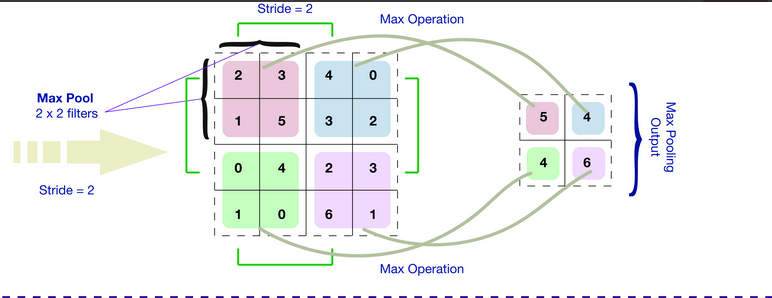
\includegraphics[width=0.8 \textwidth]{Images/maxpooling2D}}
    \caption{Overview for max pooling (Image from https://www.quora.com/What-is-max-pooling-in-convolutional-neural-networks)}
    \label{fig:Max pooling}

\end{figure}

We have also used batch normalisation with the default settings in the input and hidden layers of out model.
This means that the model is sharding the data in batches.
This in turn lets us train the model with a lot less training steps, and it gives us even better accuracy.
The last function we will talk about in the input and hidden layers are the dropout function.
This function will force the model to drop random filters during the training.
This will force an adaption in the model that makes it more versatile.
This is because the model can't just rely on one good path to carry its accuracy.
Therefore, it will end up with a more generic understanding of the data and avoid an overfitting.

\begin{figure}[h]
    \center{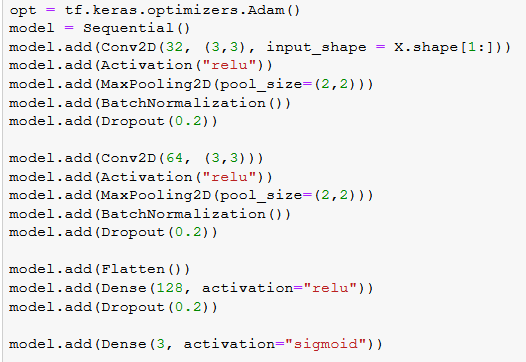
\includegraphics[width=0.8 \textwidth]{Images/CNN_model}}
    \caption{CNN model}
    \label{fig:CNN model}

\end{figure}

In the compile function we defined we choose to use cross-entropy as our loss function.
Because this is the best for multiclass classification.
The optimizer is the standard adam optimizer.

\begin{figure}[h]
    \center{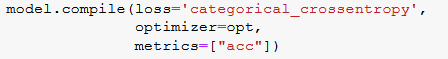
\includegraphics[width=0.8 \textwidth]{Images/CNN_compile}}
    \caption{CNN model compile}
    \label{fig:CNN compile}

\end{figure}


\section{OCR}\label{sec:OCR_implementation}

\subsection{OCR alignment}

The alignment model is made from (https://learnopencv.com/feature-based-image-alignment-using-opencv-c-python/) as a base.
We have changed this code base to fit our pipeline.
We wrapped this base code in two different functions.
Aligne\_images and return\_data.
Aligne\_images takes three parameters.
It takes the prediction form the CNN to see if it need to scale the image and it takes two images.
One of these images is the image that the user sendt in via the webpage.
The other image is the template image that the OCR is going to use to aligne the image.
The return\_data function also takes the prediction.
This decides the template image.
and it takes the image from the webpage changes the colors and passes it to align\_images

\subsection{OCR extraction}

The OCR extraction model is based on code from Murtaza's workshop (https://www.computervision.zone/courses/text-detection/).

\begin{figure}[h]
    \center{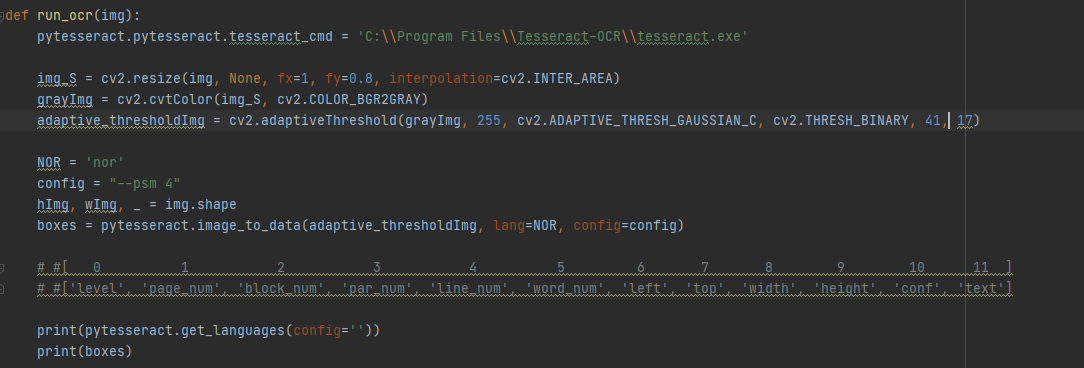
\includegraphics[width=0.8 \textwidth]{Images/OCR}}
    \caption{OCR config and thresholding}
    \label{fig:OCR config/thresholding}
\end{figure}

We wrapped the whole code in a function and made it take an image from the alignment model.
The image goes through more resizing, and the thresholding process starts.
We decided to go with a combination of adaptive gaussian\_c and binary thresholding.
As ilustrated in


\begin{figure}[h]
    \center{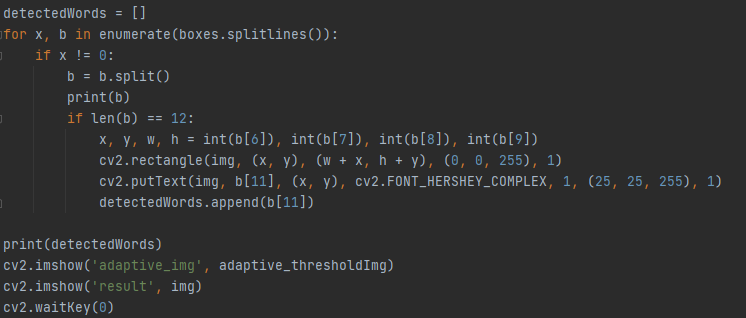
\includegraphics[width=0.8 \textwidth]{Images/OCR5}}
    \caption{OCR extraction}
    \label{fig:OCR text extraction}
\end{figure}

This is the part of the model that extracts the text.
The important things to note here is that we are casting b[6-9] to ints.
These are strings, and we cannot use strings to determined height and width of the textboxes's.
We also add b[11] to an array, because these are the words that the OCR finds.

\clearpage

\begin{figure}[h]
    \center{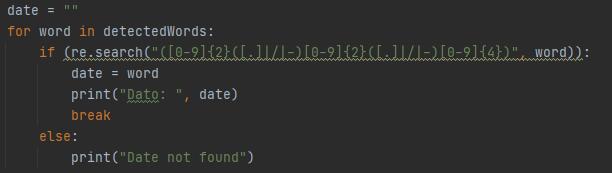
\includegraphics[width=0.8 \textwidth]{Images/OCR_dato}}
    \caption{OCR text extraction}
    \label{fig:OCR date extraction}
\end{figure}

The last thing in the model is the date validation.
We have made a simple regex that uses the pattern for dates to recognize dates.
The first match that comes up is the one we use.
